\documentclass[UTF8]{pkuthss}
\usepackage[backend = biber, style = caspervector, utf8, sorting = ecnyt]{biblatex}

% 对于 linespread 值的计算过程有兴趣的同学可以参考 pkuthss.cls。
\renewcommand*{\bibfont}{\zihao{5}\linespread{1.27}\selectfont}
\usepackage{iftex, fancyvrb, hologo}
\let\openbox\relax
\usepackage{amsthm} %数学公式
\hypersetup{colorlinks = true, allcolors = blue}
\ctexset{linestretch = 2\ccwd}
\setlength{\hfuzz}{3pt}
\setlength{\bibitemsep}{3bp}
\renewcommand*{\bibfont}{\zihao{5}\linespread{1.27}\selectfont}
\newcommand*{\cupercite}[1]{\supercite{#1}\mbox{}}
\newcommand{\myemph}[1]{\emph{\textcolor{red}{#1}}}
\newcommand{\unemph}[1]{\textup{\textcolor{black}{#1}}}
\RecustomVerbatimEnvironment{Verbatim}{Verbatim}%
{frame = single, tabsize = 4, formatcom = {\ifXeTeX\xeCJKVerbAddon\fi}}
\RecustomVerbatimCommand{\VerbatimInput}{VerbatimInput}{
	fontsize = {\small}, baselinestretch = 1,
	tabsize = 4, formatcom = {\ifXeTeX\xeCJKVerbAddon\fi}
}
\newcommand*{\docversion}{v1.8.2}
\pkuthssinfo{
	cthesisname = {}, ethesisname = {Undergraduate Thesis},
	ctitle = {英特尔$^\circledR$各代酷睿$^\text{TM}$系列微架构的变迁\\pkuthss \docversion},
	etitle = {%
		PKU dissertation document class\texorpdfstring{\\}{: }%
		pkuthss \docversion%
	},
	cauthor = {左熙辰},
	eauthor = {Zuo Xichen},
	studentid = {2000012103},
	date = {\zhdigits{2020} 年 \zhnumber{11} 月},
	school = {生命科学学院},
	cmajor = {生命科学}, emajor = {Life Science},
	direction = {},
	cmentor = {}, ementor = {},
	ckeywords = {英特尔$^\circledR$,酷睿$^\text{TM}$,架构},
	ekeywords = {Intel,Core,framework}
}
\addbibresource{article.bib}
\bibliography{article}
\begin{document}
	\maketitle
	\begin{cabstract}
		英特尔$^\circledR$作为世界上顶尖的大规模集成电路生产、制造公司,其主流消费级芯片Core$^\text{TM}$(中文译名酷睿$^\text{TM}$)系列,在一定程度上可以反映该公司的走向和芯片制造工艺历史变迁,本文将从第一代酷睿$^®$芯片开始开始,逐一介绍各代酷睿$^\circledR$系列微架构的变迁,包括制造工艺,产品代号以及部分产品的内部结构。
	\end{cabstract}
	\section{Nehalem架构}
	Nehalem架构于2008年推出,2008年初代采用45nm制程\cite{blog.csdn.net},2010年的Core Westmere采用32nm制程,是上一代Core架构的改进产品,计算内核的设计改动主要为重新采用超线程技术(极大地提升了逻辑内核的数量)、支持Turbo Boost技术$^\text{TM}$(英特尔睿频$^\text{TM}$技术)和支持SSE4.2等方面,非计算内核的设计改动主要有三级包含式Cache设计、使用QPI总线和整合内存控制器等。\cite{www.expreview.com}
	\begin{figure}[ht]
		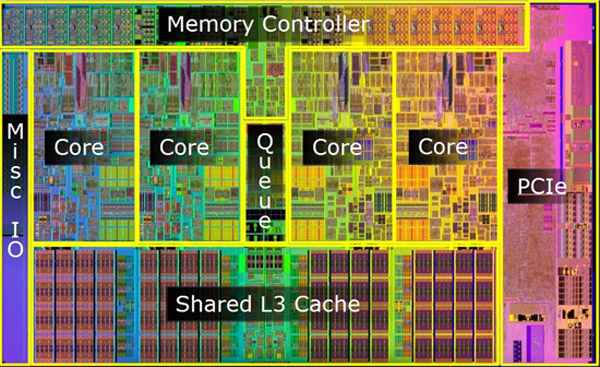
\includegraphics[scale=0.75]{lynnfield.jpg}
		\caption{基于Nehalem架构的Lynnfield核心示意图}
	\end{figure}
	
	而Nehalem架构最重要的设计就是采用了可扩展架构,这也为以后的酷睿系列在该架构的基础上有着更多的灵活性的扩展奠定了基础,例如支持三通道DDR3的Bloomfield核心、支持双通道DDR3的Lynnfield和Clarkdale核心,而且这些核心间还存在是否支持超线程、Turbo Boost技术等区别,Clarkdale还整合了GPU图形单元,而于2009年推出的Lynnfield处理器将PCI-E控制器等部分北桥芯片中的功能整合到了CPU内部,形成了一直沿用至今的主板双芯片格局。
	\section{Sandy Bridge架构}
	Sandy Bridge架构于2010年首发,采用32nm,22nm架构\cite{blog.csdn.net},它真正将GPU与CPU融合, 内核架构也较Nehalem有了较大变化,这些变化包括:新的分支预测单元、新的Uop缓存、新的物理寄存器文件、有效执行256位指令、放弃QPI总线改用环形总线、最末级缓存LLC机制等。
	
	AVX(矢量拓展指令集)的加入是Sandy Bridge最为重要的改进,浮点性能得以激增,新一代的Turbo Boost 2.0技术增强了Sandy Bridge自动提速的弹性,除CPU外还可对GFX进行加速,并随着系统负载的不同协调二者的频率升降,表现得更加智能化。
	\begin{figure}[ht]
		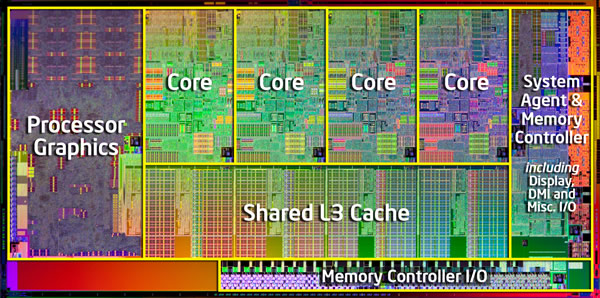
\includegraphics[scale=0.75]{Sandy-Bridge-Die-Map.jpg}
		\caption{Sandy Bridge架构示意图}
	\end{figure}
	新一代图GPU改用环形总线设计,三级缓存可由CPU各核心、GPU核心与系统助理System Agent共享,可直接在L3内进行通信。GPU主要包含了指令流处理器、媒体处理器、多格式媒体解码器、执行单元、统一执行单元阵列、媒体取样器、纹理采样器以及指令缓冲等等,架构与上一代相比有了较大修改。
	\subsection{Ivy Bridge架构}
	Ivy Bridge是Sandy Bridge的工艺改良版,架构上没太大改变,它是首次采用22nm 3D晶体管工艺,是今后Intel半导体工艺的重要基础;另外CPU内部的PCI-E控制器也升级到了PCI-E 3.0标准;内核方面的改进说是提升了IPC每周期指令性能,SSE以及AVX指令也有所增强;整合GPU性能也有所提升,EU数从12个提升到16个,API支持也从Directx10.1升级到了Directx11。
		\begin{figure}[ht]
		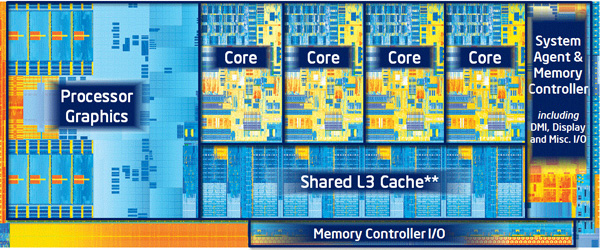
\includegraphics[scale=0.75]{ivy06.jpg}
		\caption{Ivy Bridge核心示意图}
	\end{figure}
	\section{Haswell架构}
	Haswell于2013年推出,采用22nm和14nm工艺\cite{blog.csdn.net},该架构把原来主板上的VRM模块整合到了CPU内部,FIVR调压模块的加入让主板的供电变得简单,并且可以对CPU内部的电压进行更为精确的控制,提高供电效率。
	\begin{figure}[ht]
		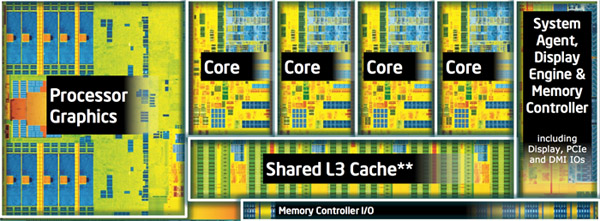
\includegraphics[scale=0.75]{Haswell.jpg}
		\caption{Haswell架构示意图}
	\end{figure}
	
	指令集方面,Haswell增加了两个指令集,一是优化多线程过程的TSX扩展指令,二是针对矢量计算的AVX2。另外,从Haswell架构开始Intel的核显开始了模块化设计,并且可以进行扩展,就此Intel开始大规模堆砌核显规格,最高级的核显拥有40个EU,还有大容量eDRAM作为L4缓存,可以同时提升CPU与GPU性能。
		\begin{figure}[ht]
		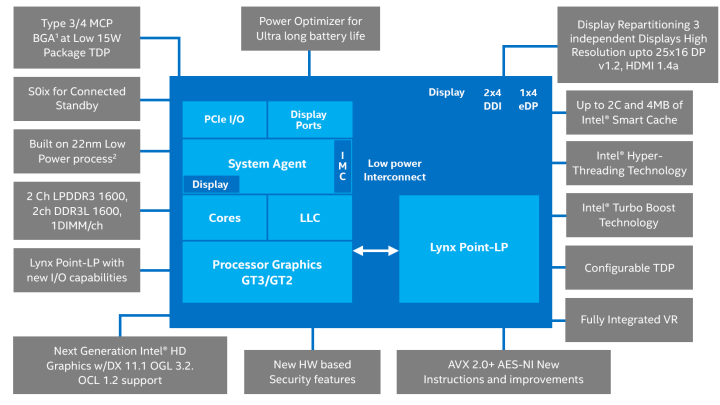
\includegraphics[scale=0.6]{haswell-uy-block-diagram-16x9.png.rendition.intel.web.720.405.png}
		\caption{Haswell-U/Y设计示意图}
	\end{figure}

	Haswell-S采用与苹果类似的SoC片上系统设计与22nm制程,主要用于移动PC(笔记本电脑等),Lynx-Point主板芯片支持了HDMI接口,添加了对VR技术的支持,\cite{www.intel.cn-haswell-u-y}而针对高性能需求的Hsawell-E系列则增加了对USB3.0的高速传输和DDR4内存支持,并放宽了对超频的限制。\cite{www.intel.cn-haswell-e}
	\section{Skylake架构}
	Skylake可以说是自Sandy Bridge以来升级幅度最大的,CPU同时升级架构、工艺及核显,内存同时支持DDR3与DDR4,采用了更为先进的14nm工艺\cite{blog.csdn.net}使得Skylake在提升频率、增强性能的同时明显降低功耗,而FIVR电压控制模块则被取消了,CPU电压也重新由主板控制。在Skylake处理器上,Intel虽然继续限制倍频,但放宽了对BCLK外频的限制。
		\begin{figure}[ht]
		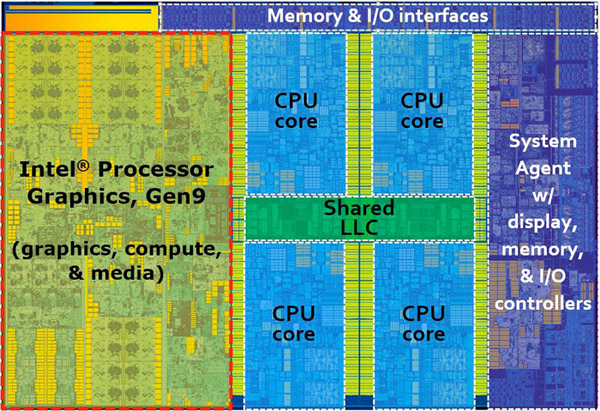
\includegraphics[scale=0.75]{Skylake.jpg}
		\caption{Skylake架构示意图}
	\end{figure}

	核显方面,Skylake与Broadwell并无较大差别,每组Subslice单元依旧是24个EU,但是整体规模变得越来越大了,Skylake最多可以扩展到3组Slice单元,也就是说最多会配备72个EU单元,因此Skylake也多出GT4这个级别的核显,并增加了对4k视频的支持。
	
	而由于Intel 10nm技术存在严重的品控问题,使得近几年以来的制程一直没有显著的提升,架构也没有发生显著的变化,一直是属于基于Skylake的更新.
	\subsection{Kaby Lake}
	
	Kaby Lake依旧使用14nm制程,但对工艺进行了改良,Kaby Lake处理器使用了更高的鳍片与更宽的栅极间距,更高的鳍片使得CPU需要的驱动电流更小,可以减少漏电概率;更宽的栅极间距会降低晶体管的密度,这样虽然需要更高的工作电压但是降低了生产的难度,另外更宽的间距使得散热性能增强,有助于降低内核温度并提高工作频率,使得Kaby Lake频率都比Skylake高但功耗则无显著变化。
	
	GPU方面Kaby Lake的核心与Skylake一样都是Gen 9,不过针对4K视频播放进行了优化,增加了H.265 Main.10、VP9 8/10-bit格式的硬件解码与编码,可大幅降低4K视频播放时的功耗,降低移动设备功耗,增加续航时间。
\specialchap{结论}
在经历了奔腾4$^\text{TM}$的惨痛失败后,Intel在Core架构上的成功使得Intel的市场份额迅速扩大,但由于10nm技术的严重失误,使得新一代架构的研发计划被一拖再拖,而此时的死对头AMD却在经历FX系列的惨痛失败后迅速推出了Ryzen R系列,一步步蚕食着Intel的市场。而未来Intel将怎样走出困局,我们拭目以待。
	\appendix
	% 排版参考文献列表。bibintoc 选项使“参考文献”出现在目录中;
	% 如果同时要使参考文献列表参与章节编号,可将“bibintoc”改为“bibnumbered”。
	\printbibliography[heading = bibintoc]
\end{document}